% Options for packages loaded elsewhere
\PassOptionsToPackage{unicode}{hyperref}
\PassOptionsToPackage{hyphens}{url}
\PassOptionsToPackage{dvipsnames,svgnames,x11names}{xcolor}
%
\documentclass[
  10pt,
]{article}
\usepackage{amsmath,amssymb}
\usepackage{iftex}
\ifPDFTeX
  \usepackage[T1]{fontenc}
  \usepackage[utf8]{inputenc}
  \usepackage{textcomp} % provide euro and other symbols
\else % if luatex or xetex
  \usepackage{unicode-math} % this also loads fontspec
  \defaultfontfeatures{Scale=MatchLowercase}
  \defaultfontfeatures[\rmfamily]{Ligatures=TeX,Scale=1}
\fi
\usepackage{lmodern}
\ifPDFTeX\else
  % xetex/luatex font selection
  \setmainfont[]{DejaVu Serif}
  \setmonofont[]{DejaVu Sans Mono}
\fi
% Use upquote if available, for straight quotes in verbatim environments
\IfFileExists{upquote.sty}{\usepackage{upquote}}{}
\IfFileExists{microtype.sty}{% use microtype if available
  \usepackage[]{microtype}
  \UseMicrotypeSet[protrusion]{basicmath} % disable protrusion for tt fonts
}{}
\makeatletter
\@ifundefined{KOMAClassName}{% if non-KOMA class
  \IfFileExists{parskip.sty}{%
    \usepackage{parskip}
  }{% else
    \setlength{\parindent}{0pt}
    \setlength{\parskip}{6pt plus 2pt minus 1pt}}
}{% if KOMA class
  \KOMAoptions{parskip=half}}
\makeatother
\usepackage{xcolor}
\usepackage[margin=18mm]{geometry}
\usepackage{longtable,booktabs,array}
\usepackage{calc} % for calculating minipage widths
% Correct order of tables after \paragraph or \subparagraph
\usepackage{etoolbox}
\makeatletter
\patchcmd\longtable{\par}{\if@noskipsec\mbox{}\fi\par}{}{}
\makeatother
% Allow footnotes in longtable head/foot
\IfFileExists{footnotehyper.sty}{\usepackage{footnotehyper}}{\usepackage{footnote}}
\makesavenoteenv{longtable}
\usepackage{graphicx}
\makeatletter
\def\maxwidth{\ifdim\Gin@nat@width>\linewidth\linewidth\else\Gin@nat@width\fi}
\def\maxheight{\ifdim\Gin@nat@height>\textheight\textheight\else\Gin@nat@height\fi}
\makeatother
% Scale images if necessary, so that they will not overflow the page
% margins by default, and it is still possible to overwrite the defaults
% using explicit options in \includegraphics[width, height, ...]{}
\setkeys{Gin}{width=\maxwidth,height=\maxheight,keepaspectratio}
% Set default figure placement to htbp
\makeatletter
\def\fps@figure{htbp}
\makeatother
\setlength{\emergencystretch}{3em} % prevent overfull lines
\providecommand{\tightlist}{%
  \setlength{\itemsep}{0pt}\setlength{\parskip}{0pt}}
\setcounter{secnumdepth}{-\maxdimen} % remove section numbering
\ifLuaTeX
  \usepackage{selnolig}  % disable illegal ligatures
\fi
\usepackage{bookmark}
\IfFileExists{xurl.sty}{\usepackage{xurl}}{} % add URL line breaks if available
\urlstyle{same}
\hypersetup{
  colorlinks=true,
  linkcolor={Maroon},
  filecolor={Maroon},
  citecolor={Blue},
  urlcolor={Blue},
  pdfcreator={LaTeX via pandoc}}

\author{}
\date{}

\begin{document}

\section{Twist torsion gives executable relation-preserving
isogenies}\label{twist-torsion-gives-executable-relation-preserving-isogenies}

All \textbf{eight} cyclic7-kernels from the p827 twist's full7-torsion
give certified rational degree7 maps from the source. Each map carries
the generator, target and complete signed relation rows with the same
scalar. This establishes a concrete connection through standard isogeny
theory. It supplies no additional information for the transported base
and establishes no solving speedup.

The fixed public source is \texttt{icv1-fp10-t5-192cb216}, y²=x³+x+15
over F827, order823, G=(2,5), Q=37G. Its d2 twist y²=x³+4x+120 has
order833 and structure C7×C119. The two groups have no common nontrivial
rational odd-order component. The new construction uses twist torsion as
isogeny kernels; it does not add twist-rational points to mixed source
relations.

The anti-Frobenius embedding is (X,Y)↦(X/2,Y·ω/4), ω²=2. Native checks
cover all49 torsion points and all2,401 pairs. Each seven-point line is
Frobenius stable. The three paired x-roots construct a normalized Vélu
map ψ(x,y)=(N/H²,yM/H³), M=N′H−2NH′. Exact polynomial curve identities,
squarefreeness, coprimality, degrees, poles and infinity are checked.
Reverse maps come from the image of the full7-torsion, followed by
inverse7 coordinate scaling. Both generic compositions equal{[}7{]};
inversion on the source subgroup is {[}588{]}∘dual since7·588=1+5·823.

\begin{longtable}[]{@{}rll@{}}
\toprule\noalign{}
Line & Quotient y²=x³+a x+b & Canonical model \\
\midrule\noalign{}
\endhead
\bottomrule\noalign{}
\endlastfoot
0 & a54,b121 & \texttt{icv1-fp10-t5-44c1ec1d} \\
1 & a211,b695 & \texttt{icv1-fp10-t5-bdd22a81} \\
2 & a27,b514 & \texttt{icv1-fp10-t5-aa4928b9} \\
3 & a11,b543 & \texttt{icv1-fp10-t5-3b71719e} \\
4 & a229,b473 & \texttt{icv1-fp10-t5-b4defb92} \\
5 & a17,b601 & \texttt{icv1-fp10-t5-abb926d8} \\
6 & a665,b221 & \texttt{icv1-fp10-t5-6c3bd6f1} \\
7 & a367,b162 & \texttt{icv1-fp10-t5-0f8036c6} \\
\end{longtable}

Every quotient has order823. Native generic checks verify16 dual
compositions; exhaustive rational checks cover6,584 forward and6,584
reverse points, including identity. Independent PARI constructs all maps
and reverse maps with \texttt{ellisogeny}, checks exact
formulas/compositions and verifies public-point recovery. Eight
corrupt-map controls are rejected.

Two fixed target-blind bases contain eight oriented points including G.
One uses ascending source coordinates; the other uses shifted
coordinates from the lexicographically first maximal-order twist seed,
order119. Each mapped base uses the actual image points with preserved
signs. All arity2/3 witnesses for Q+jG, j0--15, are enumerated:64 source
plus512 destination cases. Every index/sign witness set and resulting
coefficient matrix agrees exactly with the corresponding source base.
There are1,593 F3 checks,144 explicit identity first-pair exceptions
and954 rejected flipped-sign controls.

\begin{figure}
\centering
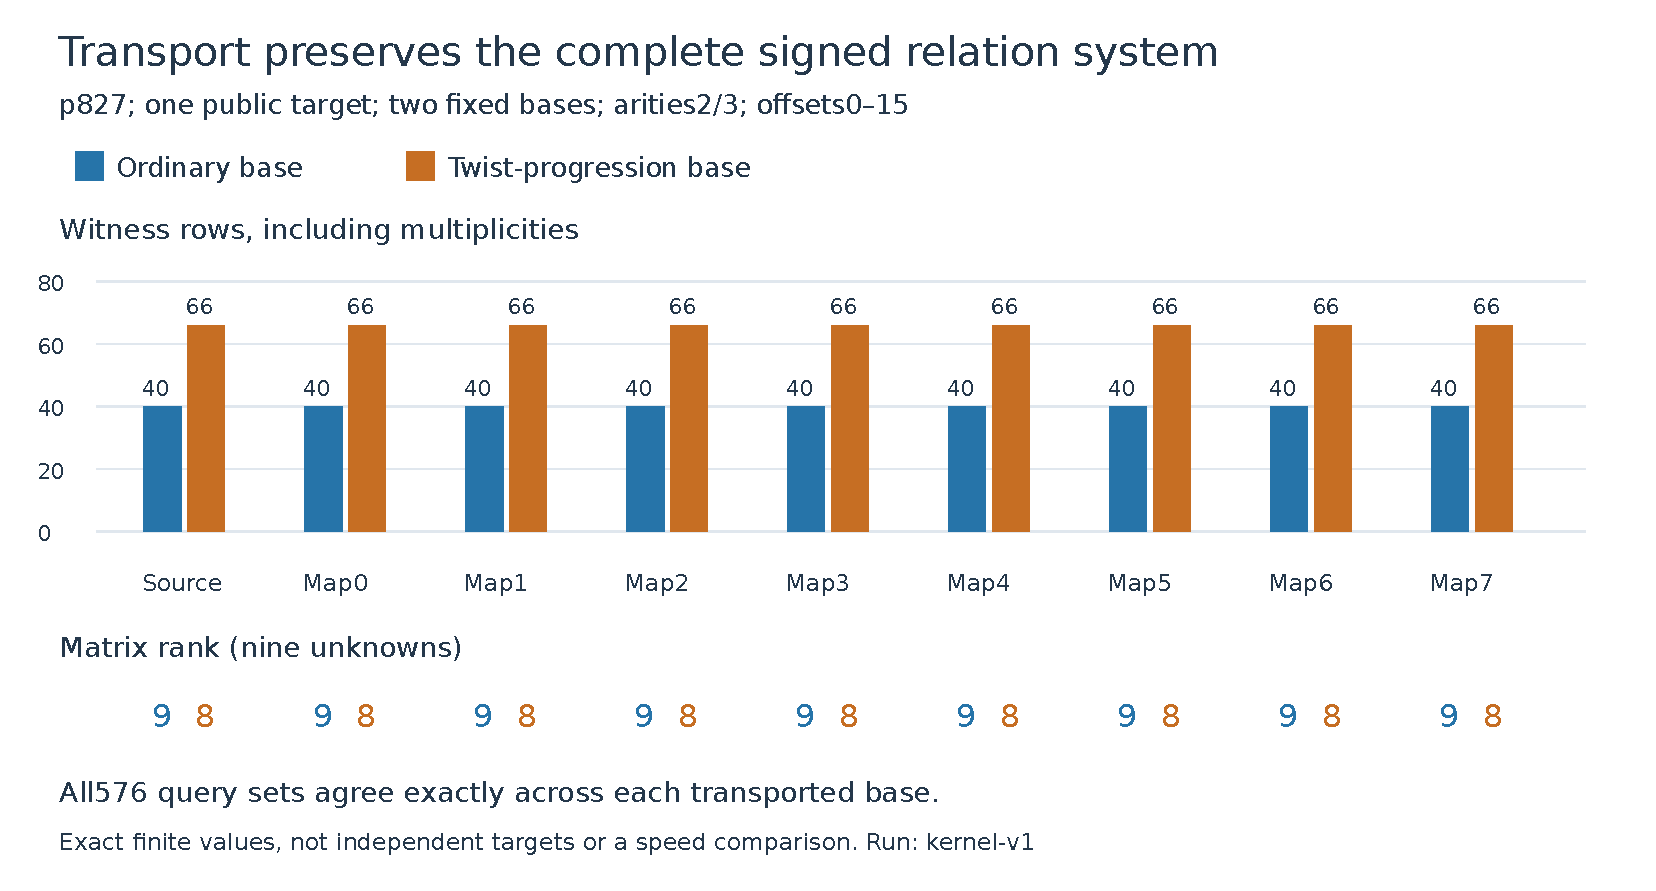
\includegraphics{SYSTEMS.pdf}
\caption{Exact signed rows and matrix ranks}
\end{figure}

The ordinary base has40 witness rows, rank9 and verified scalar37. The
twist base has66 rows but rank8; the frozen full-system solver returns
no complete solution. Counts include repeated-index/sign multiplicities,
not distinct independent rows. The
\href{../relation-rank-20261027/RESULTS.md}{separate
target-identifiability diagnostic} confirms that the twist-base target
itself remains ambiguous. All nine models retain each outcome. These are
correlated queries for one public target, not18 independent DLPs. No
factor-base logs or known37 enter elimination.

Source93a8281dbf29a51ba4be3ba57dce3d6222402bc8; frozen protocol
44d59074\allowbreak{}bd25ea25\allowbreak{}8211b1ef\allowbreak{}482cfbdd\allowbreak{}30c96bf8\allowbreak{}e74e66a4\allowbreak{}df9a541e\allowbreak{}f482d153. Native
producer and complete native replay pass; independent GP passes strict
exit/output/hash checks (only its exact declared stack-size warning).
Two whole-panel arms complete. Full protocol/export/file binding has
zero findings. Native/CAS bounds are300s each,4GiB,CPU0,one thread.
Managed Xeon Platinum8573C KVM, L0; operational timestamps are not
performance observations. The documented EKS access/image fallback
applies. No paid compute or IAM change.

Four Lean declarations check the structural group implication:
\texttt{TwistKernelRelations.recovery}, \texttt{.injective},
\texttt{.relation\_iff}, \texttt{.scalar\_transport}. They assume
additive group laws, homomorphisms, the degree7 dual identity
and823-torsion. Their proofs establish recovery, injectivity and
relation/scalar equivalence; the concrete curve/map/dual bridge is
\textbf{not formalized}. Fresh axiom audit uses only propext,
Classical.choice, Quot.sound; no custom axioms, sorry or trusted native
evaluation.

The standard descent/Vélu construction is prior art: Sutherland,
MIT18.783 Fall2025 Lecture5, Theorems5.11/5.15 and Remarks5.16--17.
Primary source and PARI help were read before implementation; atlas
isogeny/torsion obstructions were reviewed.
\href{../../execution-v8/LITERATURE.md}{Review}.

Exact \href{../../execution-v8/EC1_MODELS.json}{model manifests} retain
full curve UIDs; \href{../../execution-v8/ORDERED_ROUTES.json}{ordered
routes} bind map artifacts and direction. TWK1 identifiers are study map
IDs, not a cross-repository ISO1 certification. Eight canonical model
records and aliases are registered. No scalar map to the twist's
rational group, NIST-size route, novelty, additional transported
information, cheapest representative or full IC gain is established. No
leaderboard/benchmark row is promoted. Original campaigns and final E28
labels32--63 remain open.

Raw archive:22,024 bytes,10 members, SHA256
58618a66\allowbreak{}dfec1cbd\allowbreak{}f743d56e\allowbreak{}8d0eedde\allowbreak{}83279bb3\allowbreak{}b9906ade\allowbreak{}a1710b89\allowbreak{}f50dd768, in the
user-confirmed Setec content-addressed store. See
\href{../../execution-v8/README.md}{reproduction},
\href{../../execution-v8/ADMISSION.json}{admission},
\href{../../execution-v8/experiment.export.json}{export} and
\href{../../execution-v8/RAW_VERIFICATION.json}{archive verification}.

Next: separately freeze a cold complete decomposition cost panel on
these certified maps, with discovery/conversion charged,
source/destination same-base solver controls and ordinary group
controls. Representation choice may change equation-solving cost; exact
transport alone leaves the relation information unchanged. Existing
canonical performance graphs stay unchanged because no new performance
result was measured; this report adds a correctness diagram.

\end{document}
